%----------------------------------------------------------------------------------------
%	PACKAGES AND OTHER DOCUMENT CONFIGURATIONS
%----------------------------------------------------------------------------------------
\documentclass[12pt]{article}
\usepackage{graphicx}
\usepackage{amsmath,amsfonts,stmaryrd,amssymb} % Math packages
\usepackage{bm}
\usepackage{steinmetz}
\usepackage{enumitem}
\graphicspath{{images/}}
\usepackage{float}
\usepackage{hyperref}
\hypersetup{
	colorlinks=true,
	linkcolor=blue,
	filecolor=magenta,      
	urlcolor=cyan,
	pdftitle={Overleaf Example},
	pdfpagemode=FullScreen,
}
\urlstyle{same}
\usepackage{mathtools}
\usepackage{fancyhdr}
\usepackage{xcolor}
\usepackage[american,RPvoltages]{circuiTikz}
\usepackage{tikz, tikz-cd}
\usepackage{pgfplots}
\usepackage{siunitx}
\usetikzlibrary{spy,shapes,arrows, arrows.meta, bending, decorations.markings}
\pgfplotsset{width=10cm,compat=1.18}
\usepackage{lmodern} % package for changing font size
\usepackage{lastpage}
\renewcommand{\figurename}{Figura}
\usepackage{tcolorbox}
\usepackage{lipsum}
%\usepackage{enumerate} % Custom item numbers for enumerations
\usepackage[ruled]{algorithm2e} % Algorithms
\usepackage[framemethod=tikz]{mdframed} % Allows defining custom boxed/framed environments
\usepackage{listings} % File listings, with syntax highlighting
%\lstset{basicstyle=\ttfamily,} % Typeset listings in monospace font
\usepackage{lipsum}
\tcbuselibrary{listings,theorems,skins,vignette,raster,breakable,magazine,poster,fitting,hooks}
\usepackage[T1]{fontenc}
\usepackage{tgbonum}
 \fontfamily{garamond}
\definecolor{myblue}{RGB}{24, 51, 73}
%----------------------------------------------------------------------------------------
%	DOCUMENT MARGINS
%----------------------------------------------------------------------------------------

\usepackage{geometry} % Required for adjusting page dimensions and margins
\geometry{
	paper=a4paper, % Paper size, change to letterpaper for US letter size
	top=2.5cm, % Top margin
	bottom=3cm, % Bottom margin
	left=2cm, % Left margin
	right=2.5cm, % Right margin
	headheight=14pt, % Header height
	footskip=1.5cm, % Space from the bottom margin to the baseline of the footer
	headsep=1.2cm, % Space from the top margin to the baseline of the header
	%showframe, % Uncomment to show how the type block is set on the page
}

%----------------------------------------------------------------------------------------
%	FONTS
%----------------------------------------------------------------------------------------

\usepackage[utf8]{inputenc} % Required for inputting international characters
\usepackage[T1]{fontenc} % Output font encoding for international characters
\usepackage{XCharter} % Use the XCharter fonts
\usepackage{tgbonum}

\makeatletter
\pgfcircdeclarebipole{}{\ctikzvalof{bipoles/vsourcesin/height}}{sVpm}{\ctikzvalof{bipoles/vsourcesin/height}}{\ctikzvalof{bipoles/vsourcesin/width}}{
	
	\pgfsetlinewidth{\pgfkeysvalueof{/tikz/circuitikz/bipoles/thickness}\pgfstartlinewidth}
	\pgfpathellipse{\pgfpointorigin}{\pgfpoint{0}{\pgf@circ@res@up}}{\pgfpoint{\pgf@circ@res@left}{0}}
	\pgfusepath{draw}     
	\pgftext[bottom,rotate=90,y=\ctikzvalof{bipoles/vsourceam/margin}\pgf@circ@res@down]{\scriptsize$-$}
	\pgftext[top,rotate=90,y=\ctikzvalof{bipoles/vsourceam/margin}\pgf@circ@res@up]{\scriptsize$+$}
	
	\pgf@circ@res@up = .35\pgf@circ@res@up
	\pgfscope
	\pgftransformrotate{90}
	\pgfpathmoveto{\pgfpoint{-\pgf@circ@res@up}{0cm}}
	\pgfpathsine{\pgfpoint{.5\pgf@circ@res@up}{.4\pgf@circ@res@up}}
	\pgfpathcosine{\pgfpoint{.5\pgf@circ@res@up}{-.4\pgf@circ@res@up}}
	\pgfpathsine{\pgfpoint{.5\pgf@circ@res@up}{-.4\pgf@circ@res@up}}
	\pgfpathcosine{\pgfpoint{.5\pgf@circ@res@up}{.4\pgf@circ@res@up}}
	\pgfusepath{draw}
	\endpgfscope
}
\def\pgf@circ@sVpm@path#1{\pgf@circ@bipole@path{sVpm}{#1}}
\compattikzset{sinusoidal voltage source pm/.style = {\circuitikzbasekey, /tikz/to path=\pgf@circ@sVpm@path, \circuitikzbasekey/bipole/is voltage=true, \circuitikzbasekey/bipole/is voltageoutsideofsymbol=true, v=#1 }}
\compattikzset{sVpm/.style = {\comnpatname sinusoidal voltage source pm = #1}}

\pgfcircdeclarebipole{}{\ctikzvalof{bipoles/vsourcesin/height}}{sVpmh}{\ctikzvalof{bipoles/vsourcesin/height}}{\ctikzvalof{bipoles/vsourcesin/width}}{
	
	\pgfsetlinewidth{\pgfkeysvalueof{/tikz/circuitikz/bipoles/thickness}\pgfstartlinewidth}
	\pgfpathellipse{\pgfpointorigin}{\pgfpoint{0}{\pgf@circ@res@up}}{\pgfpoint{\pgf@circ@res@left}{0}}
	\pgfusepath{draw}     
	\pgftext[center,x=0.2\pgf@circ@res@down-\ctikzvalof{bipoles/vsourceam/margin}\pgf@circ@res@down]{\scriptsize$-$}
	\pgftext[top,rotate=90,y=\ctikzvalof{bipoles/vsourceam/margin}\pgf@circ@res@up]{\scriptsize$+$}
	
	\pgf@circ@res@up = .35\pgf@circ@res@up
	\pgfscope
	\pgftransformrotate{90}
	\pgfpathmoveto{\pgfpoint{-\pgf@circ@res@up}{0cm}}
	\pgfpathsine{\pgfpoint{.5\pgf@circ@res@up}{.4\pgf@circ@res@up}}
	\pgfpathcosine{\pgfpoint{.5\pgf@circ@res@up}{-.4\pgf@circ@res@up}}
	\pgfpathsine{\pgfpoint{.5\pgf@circ@res@up}{-.4\pgf@circ@res@up}}
	\pgfpathcosine{\pgfpoint{.5\pgf@circ@res@up}{.4\pgf@circ@res@up}}
	\pgfusepath{draw}
	\endpgfscope
}
\def\pgf@circ@sVpmh@path#1{\pgf@circ@bipole@path{sVpmh}{#1}}
\compattikzset{sinusoidal voltage source pmh/.style = {\circuitikzbasekey, /tikz/to path=\pgf@circ@sVpmh@path, \circuitikzbasekey/bipole/is voltage=true, \circuitikzbasekey/bipole/is voltageoutsideofsymbol=true, v=#1 }}
\compattikzset{sVpmh/.style = {\comnpatname sinusoidal voltage source pmh = #1}}
\makeatother


%----------------------------------------------------------------------------------------
%	BEGIN DOCUMENT
%----------------------------------------------------------------------------------------

\begin{document}
	%\thispagestyle{empty}
	\begin{tikzpicture}[remember picture, overlay]
		\node[anchor=north west, inner sep=0pt] at (current page.north west) {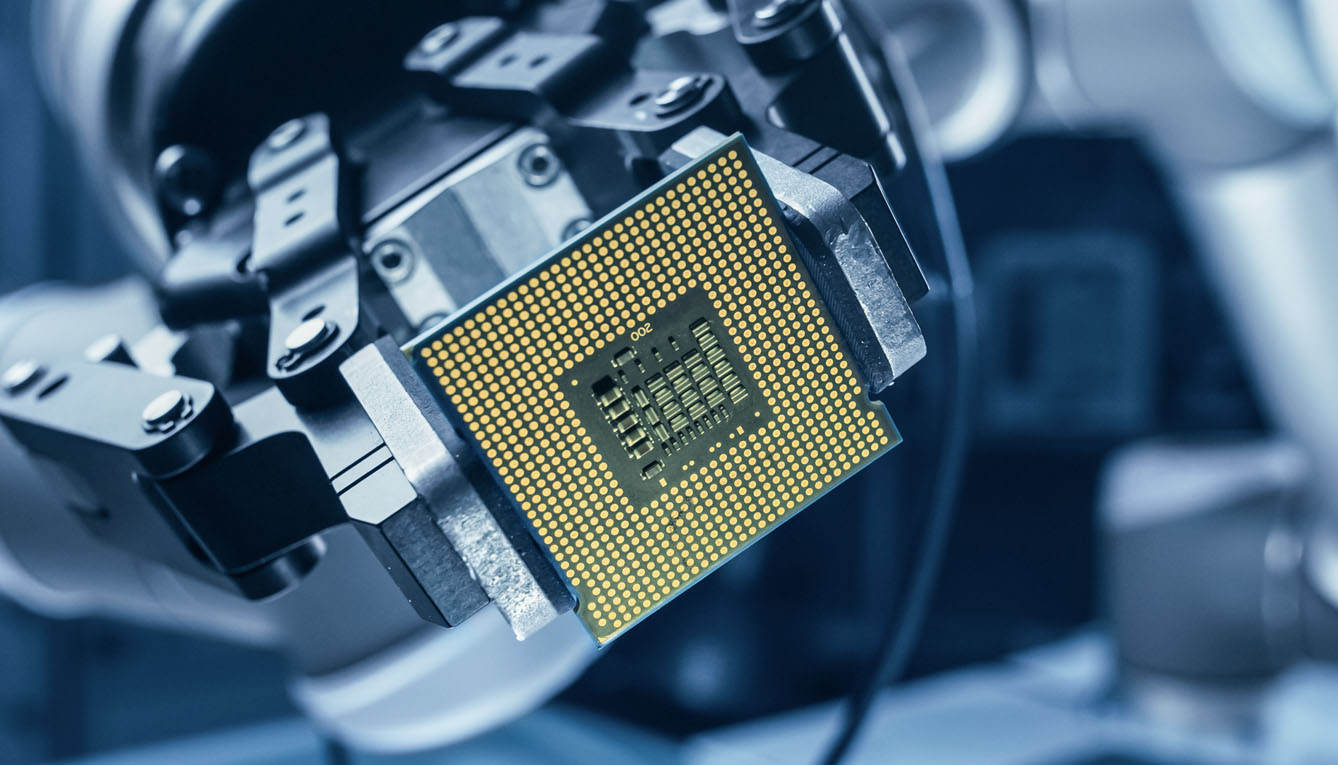
\includegraphics[width=\paperwidth, height=.5\paperheight]{picture1}};
	\end{tikzpicture}

	\vspace{13cm}
	\noindent \textcolor{myblue}{\fontsize{40pt}{40pt}\selectfont \textbf{Análisis de amplificador cascode con BJTs}}\\\\\\
	{\fontsize{18pt}{18pt}\selectfont Agosto, 2023} 
	
	\newpage
	\section*{Amplificador Cascode}
	Realice en análisis de cd y ac para el circuito de la figura 1.
	
	
	\begin{figure}[H]
		\centering	
		\begin{tikzpicture}[scale=0.8]
			\draw (0,0)   to[V, l=$v_{in}$] (0,4) coordinate(node11)
						  to[R, l=$R_{s}$] ++(3,0)
						  to[C, l=$C_1$] ++(2,0) coordinate(node1)
						  to[R, l2=$R_{3}$ and \SI{14}{\kilo\ohm}, *-*] ++(0,-4) coordinate(node3)
						  to[short] (0,0);
			\draw (node1) to[short] ++(3,0) coordinate(node2);
			\draw (node2) node[npn,right](Q1){$Q_1$};
			\draw (Q1.E)  to[R, l2=$R_E$ and \SI{0.7}{\kilo\ohm}, -*] (node3 -| Q1.E) node[ground]{} coordinate(node4) -- (node3);
			\draw (Q1.E)  to[short, *-] ++(3,0) coordinate(node5)
						  to[C, l=$C_3$] (node4 -| node5) coordinate(node9) -- (node4);
			\draw (Q1.C)  to[short] ++(0,2) coordinate(node6); 
			\draw (node6) node[npn, above left](Q2){$Q_2$};
			\draw (Q2.B)  to[short] (node1 |- Q2.B) coordinate(node7);
			\draw (node7) to[R, l2=$R_2$ and \SI{25}{\kilo\ohm}, *-] (node1);
			\draw (node7) to[C, l_=$C_4$] (node7 -| node11) node[ground]{};
			\draw (Q2.C)  to[R, l2_=$R_c$ and \SI{3}{\kilo\ohm}] ++(0,3) coordinate(node8) node[vcc]{$V_{CC}$};
			\draw (node7) to[R, l2_=$R_1$ and\SI{51}{\kilo\ohm}] (node7 |- node8) node[vcc]{$V_{CC}$};
			\draw (Q2.C)  to[C, l=$C_2$, *-] ++(6,0) coordinate(node10);
			\draw (node10)to[R, l2=$R_L$ and \SI{10}{\kilo\ohm}] (node10 |- node9)
						  to[short, -*] (node9);
			\draw (node1) node[cyan,above right]{$V_{TH1}$};
			\draw (node7) node[cyan, above right]{$V_{TH2}$};
		\end{tikzpicture}
		\caption{Amplificador cascode}	
		\label{fig:figura1}
	\end{figure}


\section*{Análisis de CD}
Para el análisis de CD, los capacitores se comportan como circuitos abiertos, por lo tanto el circuito equivalente se muestra en la figura 2.

\begin{figure}[H]
	\centering	
	\begin{tikzpicture}[scale=0.8]
		\draw (0,0) coordinate(node3)  to[R, l_=$R_3$, -*] ++(0,4) coordinate(node1)
					  to[short] ++(4,0) coordinate(node2);
		\draw (node2) node[npn, right](Q1){$Q_1$};
		\draw (Q1.E)  to[R, l=$R_E$] (Q1.E |- node3) coordinate(node8)
					  to[short] (0,0);
		\draw (Q1.C)  to[short] ++(0,2) coordinate(node4);
		\draw (node4) node[npn, above left](Q2){$Q_2$};
		\draw (Q2.B)  to[short] (Q2.B -| node1) coordinate(node6)
					  to[R, l=$R_2$] (node1);
		\draw (Q2.C)  to[R, l=$R_C$] ++(0,4) coordinate(node5) node[vcc]{$V_{CC}$};
		\draw (node6) to[R, l_=$R_1$, *-] (node6 |- node5) node[vcc]{$V_{CC}$};
		\coordinate (M) at ($(node3)!0.5!(node8)$);
		\draw (M) node[ground]{};
		\draw (M) to[short, *-] (M); 		
		\draw (node1) node[above right]{$B_1$};	
		\draw (node6) node[above right]{$B_2$};
	\end{tikzpicture}
	\caption{Circuito equivalente de CD}	
	\label{fig:figura2}
\end{figure}

Aplicando el teorema de Thévenin entre $B_1$ y tierra y entre $B_2$ y tierra, e ignorando las corrientes de base obtenemos

\begin{figure}[H]
	\centering	
	\begin{tikzpicture}[scale=0.8]
		\draw (0,0) to[V, l_=$V_{CC}$] ++(0,4)
					to[R, l=$R_1$] ++(3,0)
					to[R, l=$R_2$] ++(3,0) coordinate(node1)
					to[R, l=$R_3$] ++(0,-4) coordinate(node2)
					to[short] (0,0);
		\draw (node1) to[short, *-o] ++(2,0) coordinate(node3) node[below]{$+$};
		\draw (node2) to[short, *-o] ++(2,0) coordinate(node4) node[above]{$-$};
		\coordinate (M) at ($(node3)!0.5!(node4)$);
		\draw (M) node[]{$V_{TH}$};
		\draw (node3) ++(3,0) coordinate(node5) to[R, l=$R_1$] ++(3,0)
				to[R, l=$R_2$] ++(3,0) coordinate(node6)
				to[R, l=$R_3$] ++(0,-4) coordinate(node7)
				to[short] ++(-6,0)
				to[short] (node5);
		\draw (node6) to[short, *-o] ++(2,0) coordinate(node8);
		\draw (node7) to[short, *-o] ++(2,0) coordinate(node9);
		\coordinate (M1) at ($(node8)!0.5!(node9)$);
		\draw  [cyan, <-] (M1) node[cyan,above right]{$R_{TH}$} -- ++(1,0) ;
	\end{tikzpicture}
	\caption{Circuito equivalente de Thevenin para el nodo $B_1$}	
	\label{fig:figura3}
\end{figure}

\noindent El voltaje de Thévenin está dado por:
\begin{align}
	V_{TH1} = \frac{R_3}{R_1 + R_2 + R_3}V_{CC}
\end{align}

\noindent La resistencia equivalente de Thévenin es

\begin{align}
	R_{TH1} = R_3 \parallel (R_1 + R_2) = \frac{R_3 (R_1+  R_2)}{R_1 + R_2 + R_3}
\end{align}

\noindent Similarmente, obtenemos el voltaje y la resistencia equivalente de Thévenin entre el nodo $B_2$ y tierra

\begin{figure}[H]
	\centering	
	\begin{tikzpicture}[scale=0.7]
		\draw (0,0) to[V, l_=$V_{CC}$] ++(0,6)
		to[R, l=$R_1$] ++(6,0) coordinate(node1)
		to[R, l=$R_2$] ++(0,-3) 
		to[R, l=$R_3$] ++(0,-3) coordinate(node2)
		to[short] (0,0);
		\draw (node1) to[short, *-o] ++(3,0) coordinate(node4) node[below]{$+$};
		\draw (node2) to[short, *-o] ++(3,0) coordinate(node5) node[above]{$-$};
		\coordinate (M) at ($(node4)!0.5!(node5)$);
		\draw (M) node[]{$V_{TH}$};
		
		\draw (node4) ++(2.5,0) to[R, l=$R_1$] ++(6,0) coordinate(node6)
		to[R, l=$R_2$] ++(0,-3)
		to[R, l=$R_3$] ++(0,-3) coordinate(node7)
		to[short] ++(-6,0)
		to[short] ++(0,6);
		\draw (node6) to[short, *-o] ++(2.5,0) coordinate(node8);
		\draw (node7) to[short, *-o] ++(2.5,0) coordinate(node9);
		\coordinate (M1) at ($(node8)!0.5!(node9)$);
		\draw  [cyan, <-] (M1) node[cyan,above right]{$R_{TH}$} -- ++(1,0) ;
	\end{tikzpicture}
	\caption{Circuito equivalente de Thevenin para el nodo $B_2$}	
	\label{fig:figura4}
\end{figure}

\noindent Para el circuito de la figura 4 el voltaje de Thévenin es
\begin{align}
	V_{TH2} = \frac{R_2 + R_3}{R_1 + R_2 + R_3}V_{CC}
\end{align}

\noindent Y la resistencia equivalente de Thévenin es
\begin{align}
	R_{TH2} = R_1 \parallel (R_2 + R_3) = \frac{R_1(R_2 + R_3)}{R_1 + R_2 + R_3}
\end{align}

\noindent Así, el circuito equivalente se muestra en la figura 5
\begin{figure}[H]
	\centering	
	\begin{tikzpicture}[scale=0.8]
		\draw (0,0) node[left]{$V_{TH1}$} to[R, l=$R_{TH1}$,o-] ++(3,0)
		node[npn, right](Q1){$Q_1$};
		\draw (Q1.E) to[R, l=$R_E$, f>^=$I_E$] ++(0,-3.5) node[ground]{};
		\draw (Q1.C) to[short, f<_={$I_{C1} = I_{C2}$}] ++(0,3) node[npn, above left](Q2){$Q_2$};
		\draw (Q2.B) to[R, l_=$R_{TH2}$, -o] ++(-3,0) node[left]{$V_{TH2}$};
		\draw (Q2.C) to[R, l=$R_C$, f_<=$I_{C2}$] ++(0,3.5) node[vcc]{$V_{CC}$};
	\end{tikzpicture}
	\caption{Circuito equivalente del amplificador cascode}	
	\label{fig:figura5}
\end{figure}

\noindent Aplicando la LTK sobre la malla inferior de entrada obtenemos
\begin{align}
	V_{TH1} - R_{TH1}I_{B1} - V_{BE1} - R_{E}I_{E1} = 0
\end{align}

\noindent Sin embargo
\begin{align}
	I_B = \frac{I_C}{\beta} \quad \quad I_E = \frac{I_C}{\beta}(\beta + 1)
\end{align}

\noindent La sustitución de la ecuación (6) en (5) produce
\begin{align}
	V_{TH1} - \frac{I_{C1}}{\beta}R_{TH1} - V_{BE1} - \frac{I_{C1}}{\beta}(\beta + 1)R_{E1} = 0\\
	\frac{I_{C1}}{\beta} \left[ R_{TH1} + (\beta + 1)R_E \right] = V_{TH1} - V_{BE1} 
\end{align}

\begin{tcolorbox}[colback=red!5!white,colframe=red!75!black,arc=0mm,boxrule=0mm,width=(\linewidth+0.5cm)]
	\begin{equation}
		I_{C1} = \frac{\beta(V_{TH1} - V_{BE1})}{R_{TH1} + (\beta + 1)R_E}
	\end{equation}
\end{tcolorbox}

\noindent La corriente de emisor a través del transistor $Q_1$ es:
\begin{tcolorbox}[colback=red!5!white,colframe=red!75!black,arc=0mm,boxrule=0mm,width=(\linewidth+0.5cm)]
	\begin{equation}
		I_{E1} = \frac{I_{C1}}{\beta}(\beta +1)
	\end{equation}
\end{tcolorbox}

De acuerdo con el circuito de la figura 5
\begin{align}
	I_{C1} = I_{E2} = \frac{I_{C2}}{\beta}(\beta + 1)
\end{align}

\noindent Por lo tanto, la corriente de colector a través del transistor $Q_2$ es:
\begin{tcolorbox}[colback=red!5!white,colframe=red!75!black,arc=0mm,boxrule=0mm,width=(\linewidth+0.5cm)]
	\begin{equation}
		I_{C2} = \frac{\beta}{\beta + 1}I_{E2}
	\end{equation}
\end{tcolorbox}

\noindent El voltaje en el colector de $Q_2$ está dado por
\begin{align}
	V_{C2} = V_{CC} - R_CI_{C2}
\end{align}

\noindent El voltaje en el emisor de $Q_2$ o en el colector de $Q_1$ está dado por:
\begin{align}
	V_{TH2} - R_{TH2}I_{B2} - V_{BE2} = V_{E2} = V_{C1}\\
	V_{TH2} - R_{TH2}\frac{I_{C2}}{\beta} - V_{BE2} = V_{E2} = V_{C1}
\end{align}

\noindent Por lo tanto
\begin{align}
	V_{CE2	} = V_{C2} - V_{E2}
\end{align}

Al sustituir la ecuación (13) y (15) en (16) obtenemos
\begin{align}
	V_{CE2} = V_{CC} - R_C I_{C2} - \left( V_{TH2} - R_{TH2}\frac{I_{C2}}{\beta} - V_{BE2} \right)\\
	V_{CE2} = V_{CC} - R_C I_{C2} - V_{TH2} + R_{TH2}\frac{I_{C2}}{\beta} + V_{BE2}
\end{align}

\begin{tcolorbox}[colback=red!5!white,colframe=red!75!black,arc=0mm,boxrule=0mm,width=(\linewidth+0.5cm)]
	\begin{equation}
		V_{CE2} = V_{CC} + V_{BE2} - V_{TH2} + \left( \frac{R_{TH2}}{\beta} - R_C \right)I_{C2}
	\end{equation}
\end{tcolorbox}

\noindent El voltaje en el emisor de $Q_1$ está dado por
\begin{align}
	V_{E1} = R_E I_{E1}
\end{align}

\noindent Así, el voltaje $V_{CE1}$ está dado por
\begin{align}
	V_{CE1} = V_{C1} - V_{E1}
\end{align}

\noindent Sustituimos las ecuaciones (15) y (10) en (21)
\begin{tcolorbox}[colback=red!5!white,colframe=red!75!black,arc=0mm,boxrule=0mm,width=(\linewidth+0.5cm)]
	\begin{equation}
		V_{CE1} = V_{TH2} - \frac{I_{C2}}{\beta}R_{TH2} - V_{BE2} - \frac{I_{C1}}{\beta}(\beta + 1)R_E
	\end{equation}
\end{tcolorbox}


\section*{Análisis de CA}
Para analizar el circuito en corriente alterna, las fuentes de voltaje de dc se comportan como un cortocircuito al igual que los capacitores. Así, el circuito equivalente para AC se muestra en la figura 6.

\begin{figure}[H]
	\centering	
	\begin{tikzpicture}[scale=0.7]
		\draw (0,0)    to[sVpm, invert, l=$V_{in}$] ++(0,4)
					   to[R, l=$R_s$, a=\SI{100}{\ohm}] ++(4,0) coordinate(node1)
					   to[R, l2=$R_2$ and \SI{25}{\kilo\ohm}] ++(0,-4) coordinate(node2)
					   to[short] (0,0);
		\draw (node1)  to[short, *-*] ++(4,0) coordinate(node3)
					   to[R, -*, l2=$R_3$ and \SI{14}{\kilo\ohm}] ++(0,-4) coordinate(node4)
					   to[short, -*] (node2);
		\draw (node3)  to[short] ++(3,0) node[npn, right](Q1){$Q_1$};
		\draw (Q1.E)   to[short, -*] (Q1.E |- node4) coordinate(node5) node[ground]{} -- (node4);
		\draw (Q1.C)   to[short] ++(0,1.5)
					   to[short] ++(2,0) node[npn, rotate=90, yscale=-1,above left](Q2){};
		\coordinate (M) at ($(Q2.E)!0.5!(Q2.C)$);
		\draw (M) node[above]{$Q_2$};
		\draw (Q2.B)   to[short, -*] (Q2.B |- node5) coordinate(node6) -- (node5);
		\draw (Q2.C)   to[short, -*] ++(2,0) coordinate(node7)
					   to[R, l2=$R_C$ and \SI{3.3}{\kilo\ohm}, -*] (node7 |- node6) coordinate(node8) -- (node6);
		\draw (node7)  to[short] ++(3,0) coordinate(node9);
		\draw (node9)  to[R, l2=$R_L$ and \SI{10}{\kilo\ohm}] (node9 |- node8) -- (node8);
	\end{tikzpicture}
	\caption{Circuito equivalente de CA}	
	\label{fig:figura6}
\end{figure}

\noindent El circuito híbrido equivalente se muestra en la figura 7
\begin{figure}[H]
	%\centering	
	\begin{tikzpicture}[scale=0.7]
		\draw (0,0)    to[sVpm, invert, l_=$V_{in}$] ++(0,4)
		to[R, l=$R_s$] ++(3,0) coordinate(node1)
		to[R, l=$R_2$] ++(0,-4) coordinate(node2)
		to[short] (0,0);
		\draw (node1) to[short, *-*] ++(3,0) coordinate(node3)
		to[R, l=$R_3$] ++(0,-4) coordinate(node4)
		to[short, *-*] (node2);
		\draw (node3) to[short] ++(3,0)
		to[R, l=$r_{\pi 1}$, v=$v_{\pi 2}$] ++(0,-4) coordinate(node5)
		to[short] (node4);
		\draw (node5) to[short, *-*] ++(4.5,0)
		to[cI, invert, l=$g_{m1}v_{\pi 1}$] ++(0,4)
		to[short, -*] ++(3,0) coordinate(node6)
		to[R, l=$r_{\pi 2}$, v>=$v_{\pi 2}$, f<^=$i_{b2}$, -*] ++(0,-4) coordinate(node7) to[short] ++(-3,0);
		\draw (node6) to[cI, invert, -*, l=$g_{m2}v_{\pi 2}$] ++(4,0) coordinate(node8)
		to[R, l=$R_C$] ++(0,-4)
		to[short] ++(-4,0);
		\draw (node8) to[short] ++(3,0)
		to[R, l_=$R_L$] ++(0,-4)
		to[short, -*] ++(-3,0);
		\draw (node3) node[above]{$V_{B1}$};
		\draw (node6) node[above]{$V_{C1-E2}$};
	\end{tikzpicture}
	\caption{Circuito equivalente de CA}	
	\label{fig:figura7}
\end{figure}

\noindent El voltaje de salida $v_o$ está dado por
\begin{align}
	v_o = -g_{m2}v_{\pi 2} (R_C \parallel R_L)
\end{align}

\noindent Al aplicar la LCK sobre el nodo $V_{C1 - E2}$ obtenemos
\begin{align}
	g_{m2}v_{\pi 2} + i_{b2} = g_{m1}v_{\pi 1} 
\end{align}

\noindent O bien
\begin{align}
	g_{m2}v_{\pi 2} + \frac{v_{\pi 2}}{r_{\pi 2}} = g_{m1}v_{\pi 1}\\
	\left[ g_{m2} + \frac{1}{r_{\pi 2}} \right]v_{\pi 2} = g_{m1}v_{\pi 1}\\
	\left[  \frac{1 + g_{m2}v_{\pi 2} }{ r_{\pi 2} } \right]v_{\pi 2} = g_{m1}v_{\pi 1}
\end{align}

\begin{tcolorbox}[colback=red!5!white,colframe=red!75!black,arc=0mm,boxrule=0mm,width=(\linewidth+0.5cm)]
	\begin{equation}
		v_{\pi 2} = g_{m1}v_{\pi 1} \left( \frac{ r_{\pi 2} }{ 1 + g_{m2}v_{\pi 2} }  \right) 
	\end{equation}
\end{tcolorbox}

\noindent Sin embargo
\begin{align}
	v_{\pi 1} = \left( \frac{ r_{\pi 1} \parallel R_2 \parallel R_3 }{ R_s + r_{\pi 1} \parallel R_2 \parallel R_3  } \right)v_s 
\end{align}

\noindent Sustituyendo la ecuación (29) en (28) obtenemos
\begin{align}
	v_{\pi 2} = g_{m1}\left( \frac{ r_{\pi 2} }{ 1 + g_{m2}v_{\pi 2} }  \right) \left( \frac{ r_{\pi 1} \parallel R_2 \parallel R_3 }{ R_s + r_{\pi 1} \parallel R_2 \parallel R_3  } \right)v_s
\end{align}
 
 \noindent Para obtener la ganancia de voltaje general sustituimos la ecuación (30) en la ecuación (23)
\begin{tcolorbox}[colback=red!5!white,colframe=red!75!black,arc=0mm,boxrule=0mm,width=(\linewidth+0.5cm)]
	\begin{equation}
		A_v = \frac{v_o}{v_s}= -g_{m1}g_{m2} \left( \frac{ r_{\pi 2} }{ 1 + g_{m2}v_{\pi 2} }  \right) \left( \frac{ r_{\pi 1} \parallel R_2 \parallel R_3 }{ R_s + r_{\pi 1} \parallel R_2 \parallel R_3  } \right)\left( R_C \parallel R_L \right)
	\end{equation}
\end{tcolorbox}
 
 \noindent Donde
 
 \begin{align}
 	g_m = \frac{I_C}{V_T} \quad \quad r_{\pi} = \beta \frac{V_T}{I_C}
 \end{align}
 
\begin{align}
	N = \frac{(128)(R_{WB} - R_W)}{R_{AB}} 
\end{align}
 

\end{document}
